\documentclass{beamer}

\usepackage[english]{babel}
\usepackage[utf8x]{inputenc}
\usepackage{amsmath,amsfonts,amssymb}


\usepackage{subcaption}

\usepackage[absolute,overlay]{textpos}





\newcommand{\todo}[1]{\textcolor{red}{TODO: #1}}

\addtobeamertemplate{navigation symbols}{}{%
    \usebeamerfont{footline}%
    \usebeamercolor[fg]{footline}%
    \hspace{1em}%
    \insertframenumber/\inserttotalframenumber
}

\setbeamertemplate{bibliography item}[text]
\bibliographystyle{unsrt}


\usetheme{Luebeck}
\usecolortheme{orchid}

\title{Current state of master thesis}
\subtitle{Simulation of DSC measuring process and \\ parameter estimation of specific heat capacity $c_p$}
\author{Jan Lammel}

\begin{document}
	
\frame{\titlepage}

\frame{
	\frametitle{Table of contents}
	\tableofcontents[hideallsubsections]
	
}

\section{Introduction}
\frame{
\frametitle{Introduction}

	\begin{textblock}{7}(1,5)
		\includegraphics[width=1.0\textwidth]{/home/argo/masterarbeit/thesis/images/handwaermer[wiki].jpg}
	\end{textblock}
	
	\begin{textblock}{8}(8,5)
	\begin{itemize}
		\item We examine so called phase change materials (PCM).
		\item Important property is the heat capacity $c_p$: When does it melt and how much energy fits into?
	\end{itemize}
	\end{textblock}

	\begin{textblock}{14}(1,11.5)
	\begin{itemize}
		\item \textbf{Goal:} Simulation of measuring process to obtain specific heat capacity $c_p$ of phase change material (PCM) by parameter estimation.
	\end{itemize}
	\end{textblock}
	

}

\section{Physics}
\subsection{Important physical quantities}
\frame{
	\frametitle{Important physical quantities}
	
	\begin{textblock}{14}(1,5)
		\begin{itemize}
			\item Heat $Q$, \qquad $[Q] = J$ \\
			Amount of energy transferred because of temperature difference \\ \vspace{0.2cm}
			\item heat flux density $\Phi_q$, \qquad$[\Phi_q] = \frac{W}{m^2}$ \\
			Rate of energy transferred per unit area \vspace{0.2cm}
			\item specific heat capacity $c_p$, \qquad $[c_p] = \frac{J}{kg \cdot K}$ \\
			Material specific amount of energy needed to raise the temperature of $1kg$ by $1K$.
			
		\end{itemize}
	\end{textblock}
	
}


\subsection{Differential Scanning Calorimetry (DSC)}
\frame{
	\frametitle{Differential Scanning Calorimetry (DSC)}
	
	\begin{textblock}{15}(0.4,4)
		\centering
		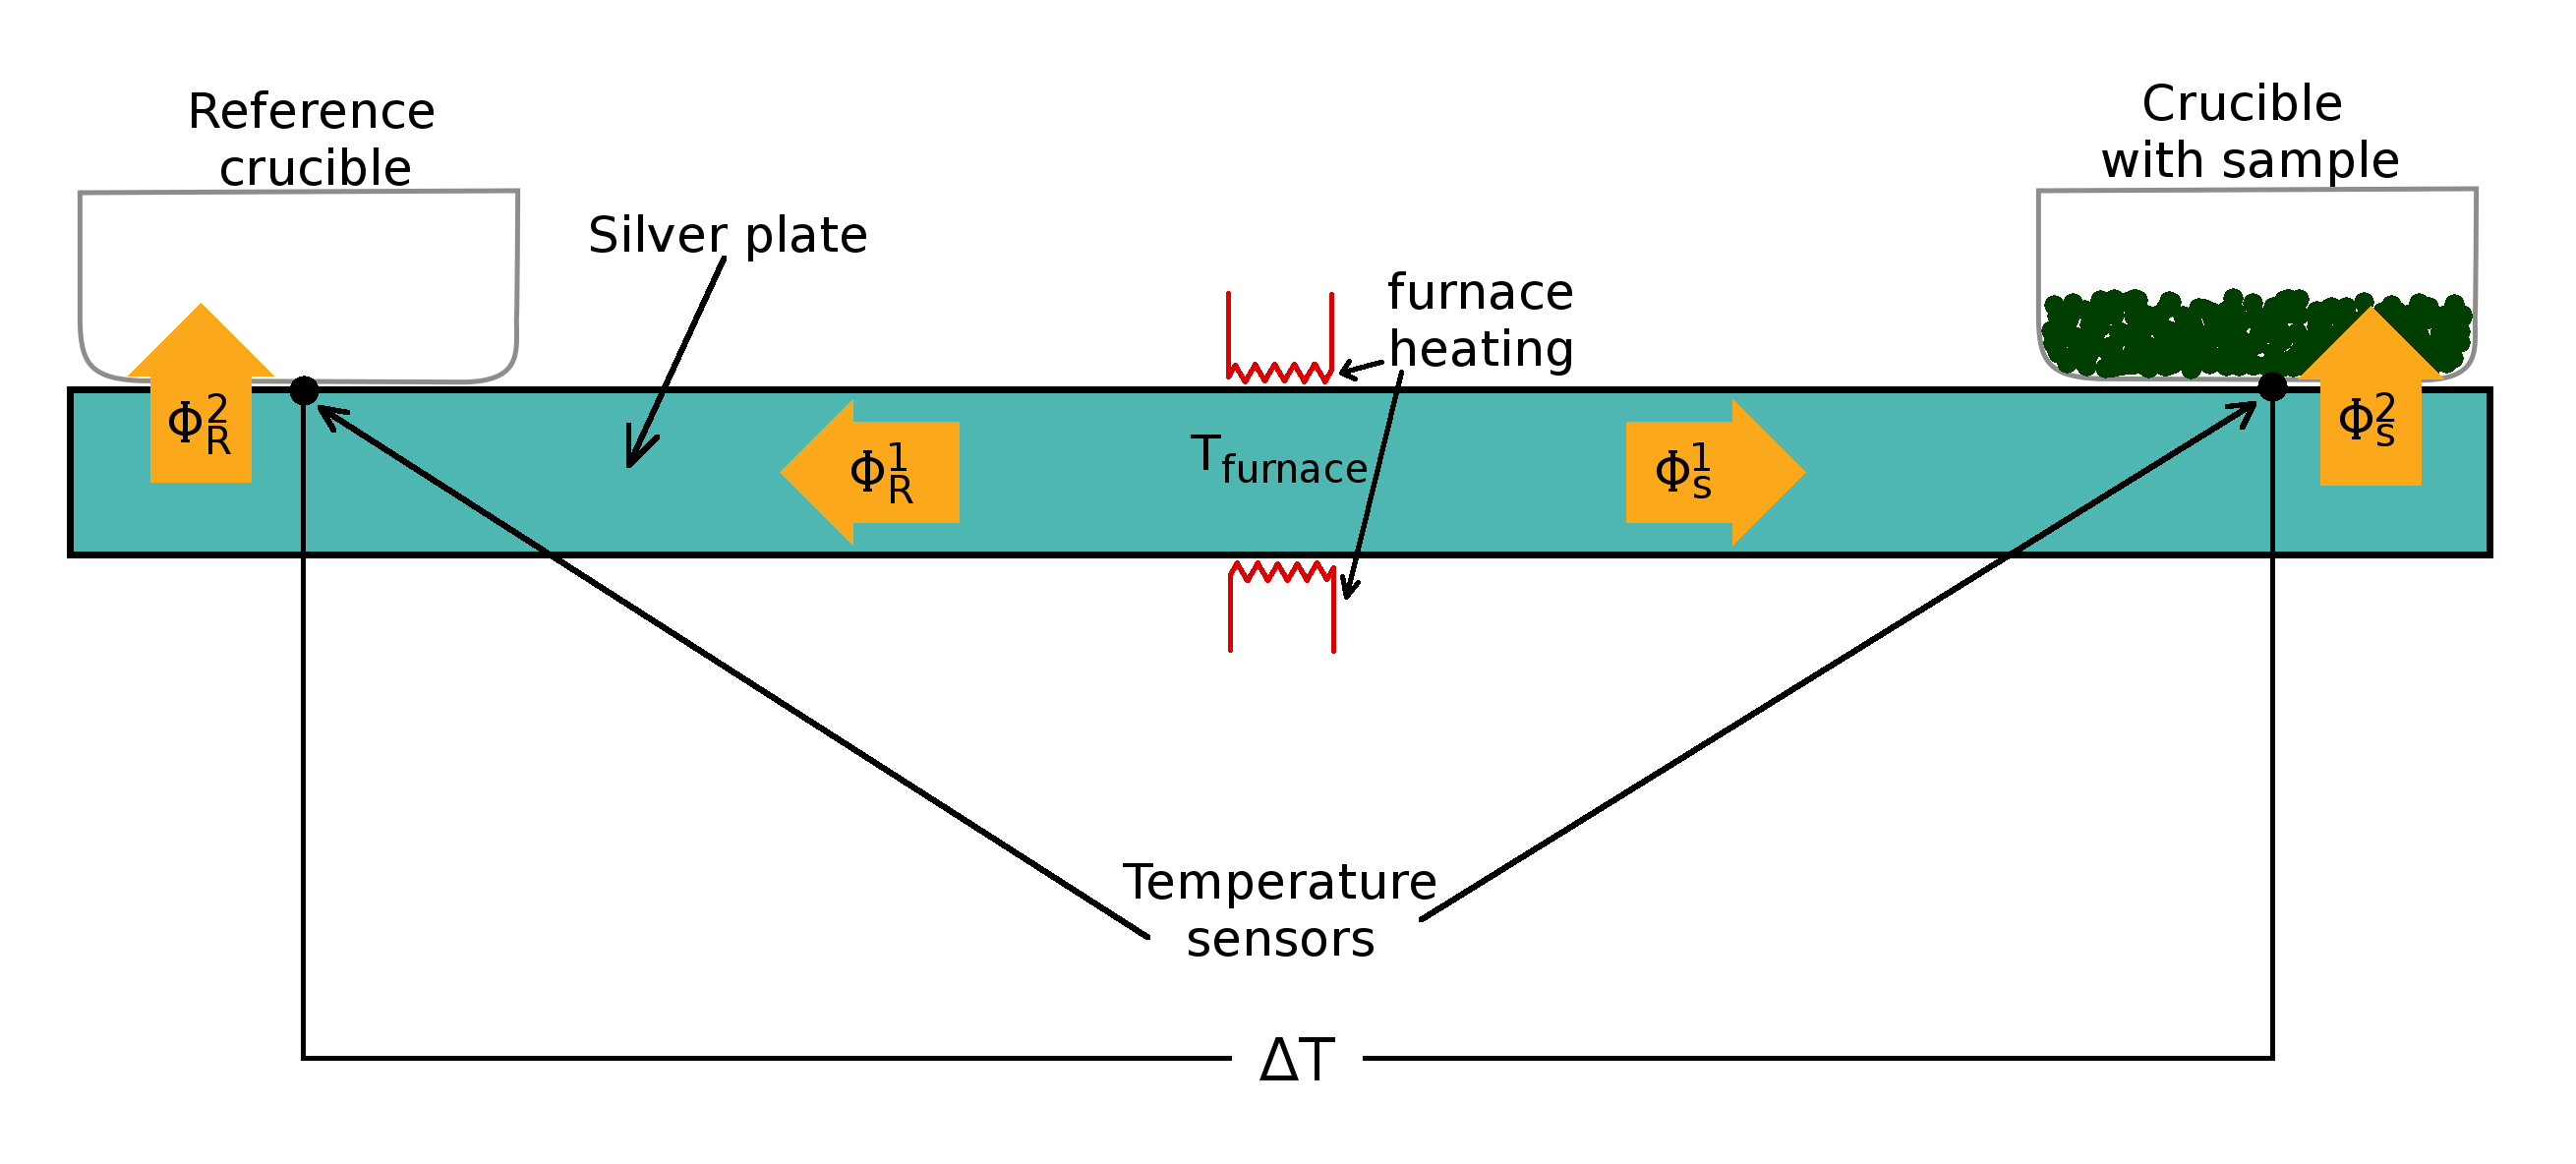
\includegraphics[width=0.7\textwidth]{/home/argo/masterarbeit/thesis/images/dsc_funktionsprinzip.png}
		
		\begin{itemize}
			\item Empty reference crucible and crucible with PCM are heated equally.
			\item Due to thermal properties differences (mainly $c_p$) of reference and PCM a temperature difference $\Delta T$ is induced.
			\item A calibration measurement with known thermal properties provides mapping $\Delta T \rightarrow \Phi_q$
		\end{itemize}
		
	\end{textblock}
	
}


\section{Parameter Estimation}
\subsection{Mathematical model}
\frame{
	\frametitle{Mathematical model}
	
	\begin{textblock}{14}(1, 4.)
		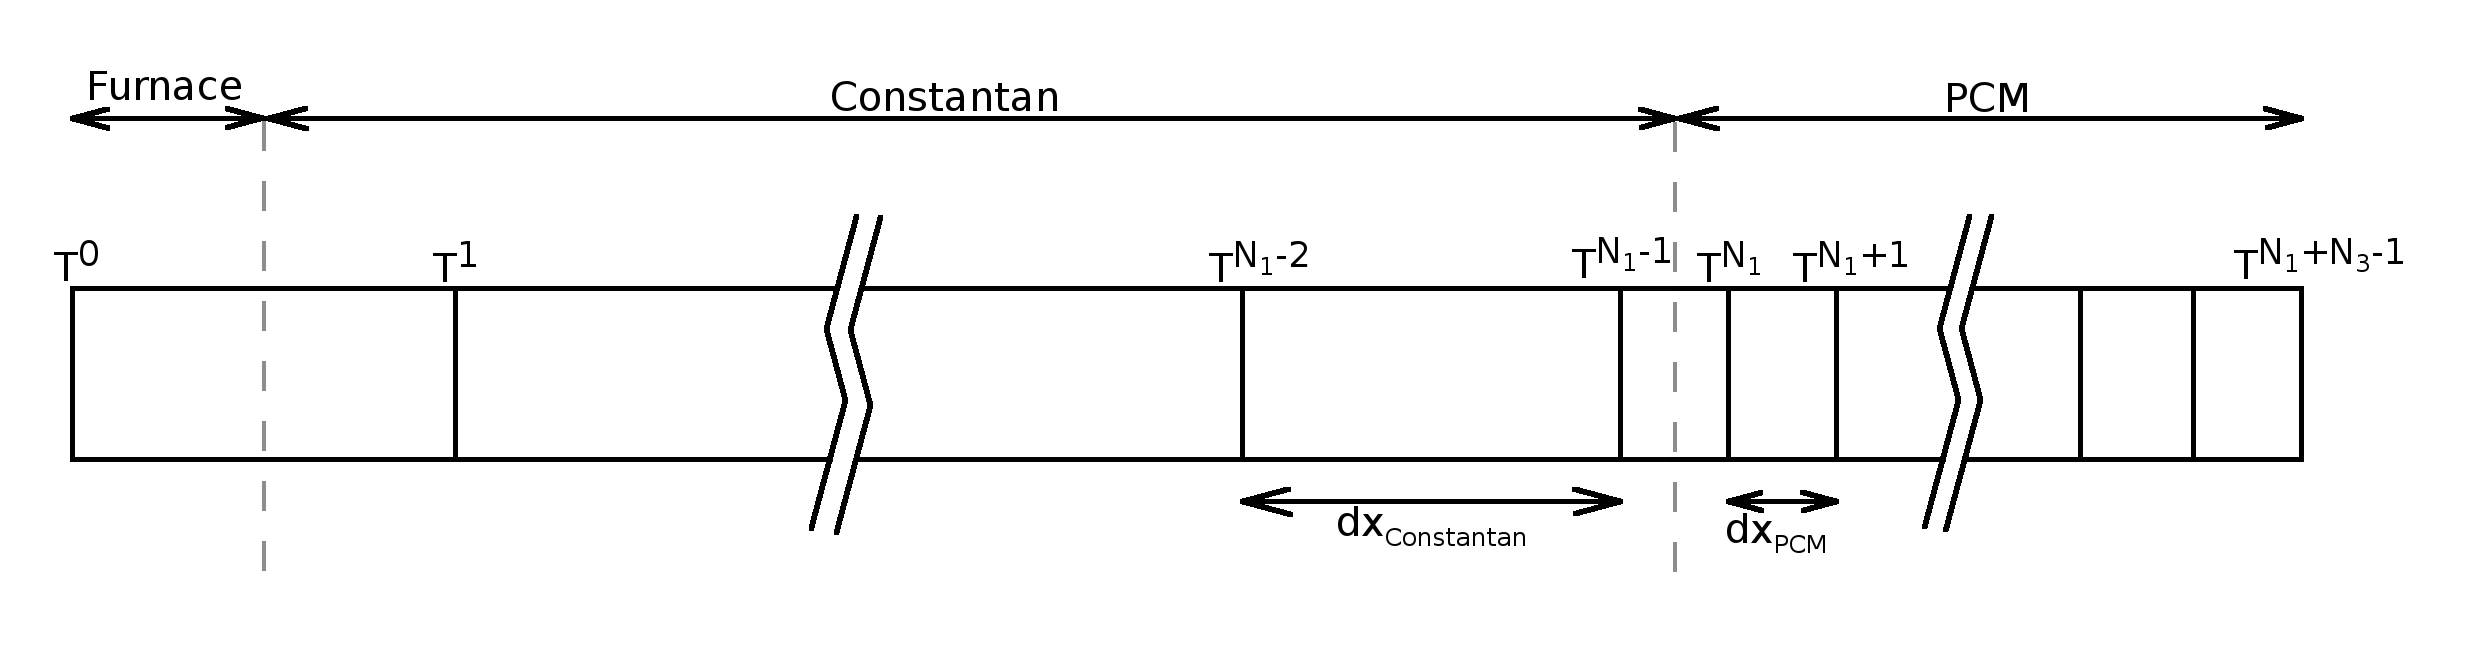
\includegraphics[width=1.\textwidth]{/home/argo/masterarbeit/thesis/images/discretization_grid.png}
	\end{textblock}
	
	
	\begin{textblock}{14}(1, 9)
	
		\begin{itemize}
			\item Heat equation: \quad $\rho c_p \frac{\partial T}{\partial t}(x,t) = \nabla \cdot \left[ \lambda \cdot \nabla T(x,t) \right]$
			\item $\rho$, $\lambda$ constant
			\item Boundary Conditions: 
				\begin{itemize}
				\item $T^0 = T_{\text{start}} + \beta \cdot t$ \\
				\item No flux outside PCM
				\end{itemize}
			\item Reference and PCM side are independent
			
		\end{itemize}
	\end{textblock}

	
}


\frame{
	\frametitle{Mathematical model}

	\begin{textblock}{14}(1, 5.)

	\begin{itemize}
		\item \todo{fehlt noch was zum modell?}
	\end{itemize}

	\end{textblock}
	
	
	
}


\subsection{Parametrization $c_p$}
\frame{
	\frametitle{Parametrization $c_p$}
	
	\begin{textblock}{14}(1,5)
		
		\begin{equation*}
			c_p(T) = \sum_{i=1}^{10} A_i \exp\left(- \frac{(T - T_{\text{offset}_i})^2}{\sigma_i^2}\right) + m \cdot T + b
		\end{equation*}
		
		\centering
		\includegraphics[width=0.5\textwidth]{/home/argo/masterarbeit/fits_data/2017-10-05_00:14:13_407_0,3Kmin_L1=15_L3=0,35/c_p(T).jpg}
		
	\end{textblock}
	
}


\subsection{Heat flux computation}
\frame{
	\frametitle{Heat flux computation}	

	\begin{textblock}{14}(1,5)
		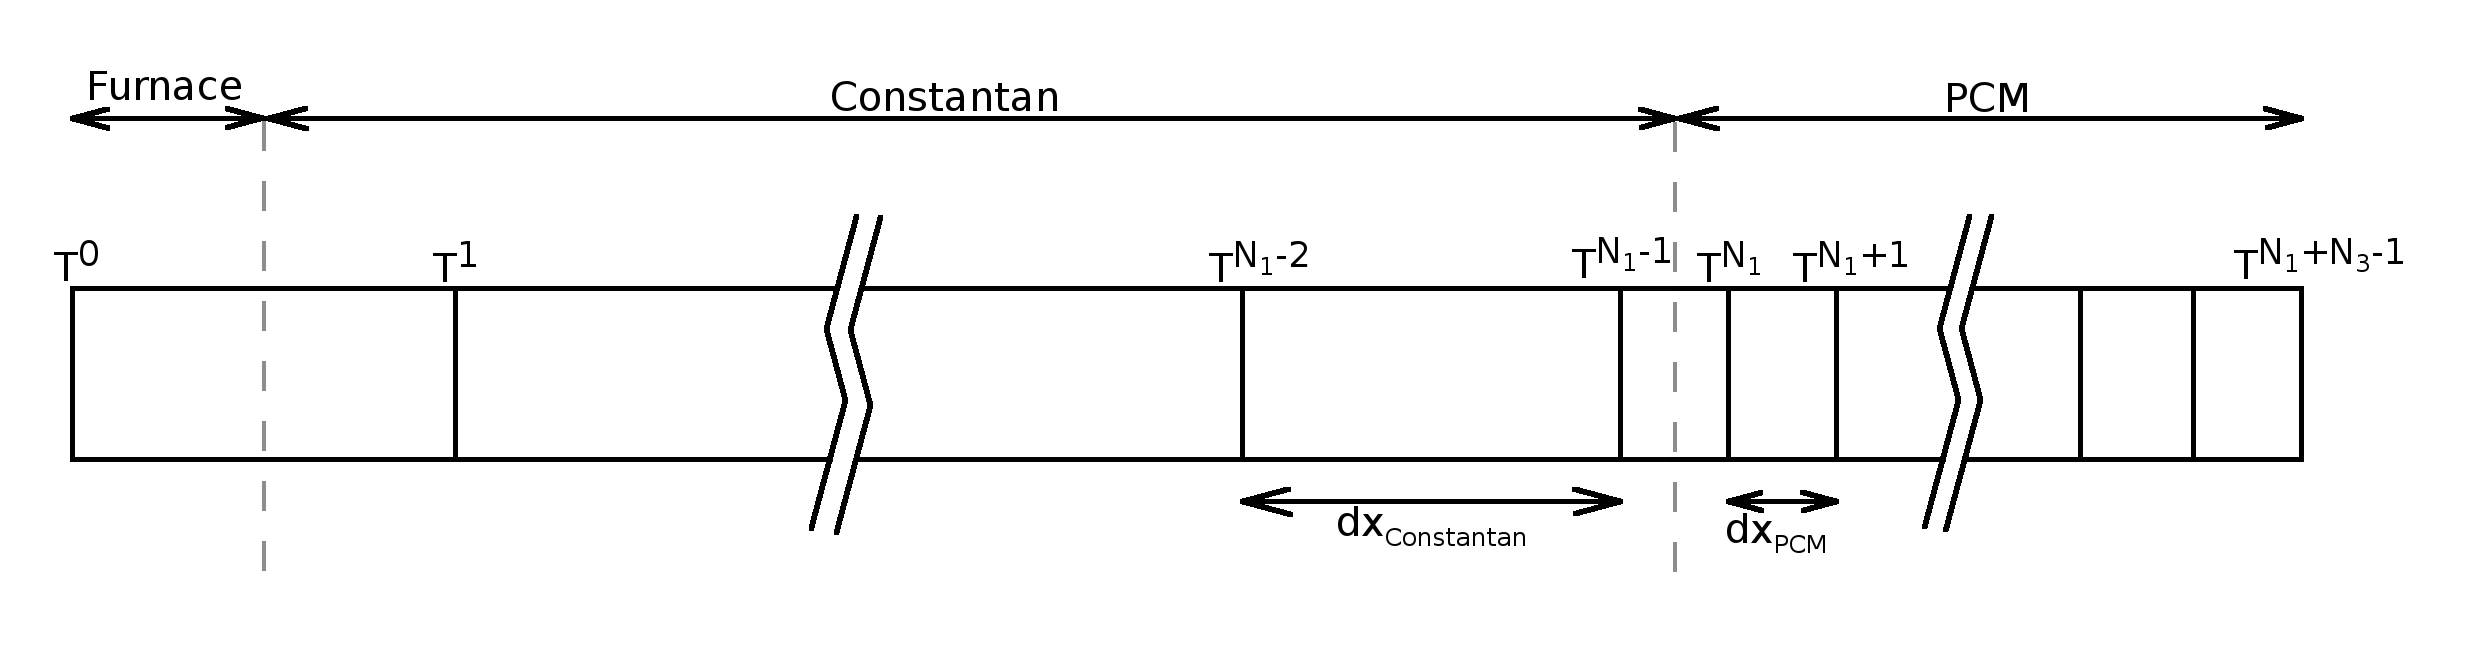
\includegraphics[width=1.\textwidth]{/home/argo/masterarbeit/thesis/images/discretization_grid.png}
	\end{textblock}
	
	\begin{textblock}{14}(1, 10)
		\begin{itemize}
			\item Heat flux into PCM: $\Phi_{q}^{PCM,in} = \bar{\lambda} \frac{T^{N_1} - T^{N_1-1}}{dx_{PCM}} \approx \lambda_{PCM} \frac{T^{N_1+1} - T^{N_1}}{dx_{PCM}}$
		\end{itemize}
	\end{textblock}


}

\subsection{Optimization problem}
\frame{
	\frametitle{Optimization problem}	

	\begin{textblock}{14}(1,5)
	\begin{align*}
		\min_{p_{c_p}} \ & \sum_{i=1}^{n_{MP}} \left|\left|  \Phi_{q}^{PCM,in}(T(t_i;T_0,p_{c_p})) - \eta_i^{\Phi} \right|\right|_2^2 \\
		s.t. \ & \quad \  \dot{T} = f(T,t;p_{c_p}) \\
		       & T(0) = T_0
	\end{align*}
	
	\begin{itemize}
		\item $\eta_i^{\Phi}$: heat flux measurement value at time $t_i$
	\end{itemize}
	
	\end{textblock}

	
}





\subsection{Results}
\frame{
	\frametitle{Results}


	\begin{itemize}
		\item Waermestrom-Fit Residuum + zugehoeriges $c_p$ fuer vllt 2, 3 versch. Heizraten
		\item In einem plot alle $c_p$ Kurven fuer alle Heizraten um Shift zu zeigen
	\end{itemize}

	
}


\section{Next potential steps}
\frame{
	\frametitle{Next potential steps}
	
	\begin{itemize}
		\item Heat equation with $\rho=\rho(T)$ \\
		$\rightarrow$ problem with value of absolute enthalpy term
		\item $L_1$ and $L_3$ as optimization variable. \\
		$\rightarrow$ huge programming effort
		\item Crucible part between Constantan and PCM. \\
		$\rightarrow$ We do not know $L_2$
		\item Solve Reference and PCM part in one system. \\
		$\rightarrow$ Implementation of sensitivity generation unclear.
	\end{itemize}
	
}



\section{Open Questions}
\frame{
	\frametitle{Open Questions}
	
	\begin{itemize}
		\item Reason for shift in $c_p$ fits?
		\item Heat equation derivation with $\rho=\rho(T)$ correct?
		\item How to get $L_1$ and $L_3$ except from optimization?
	\end{itemize}
	
}





	
	
\end{document}